% chktex-file 46
% chktex-file 3

\section*{Problem 1}
\textbf{Collaborators:} Indu Ramesh.
\medskip

We will use the identity (thanks to Indu) that
\begin{align}\label{eq:induid}
    \norm{x-y}^2 &= \sum_{i=1}^d(x-y)^2
    = \sum_{i=1}^d (x^2 -2xy + y^2)
    \nonumber \\
    &= \sum_{i=1}^d x^2 + \sum_{i=1}^d y^2 -
    2 \sum_{i=1}^d xy \nonumber \\
    &= \norm{x}^2 + \norm{y}^2 - 2\braket{x}{y}
\end{align}
which also gives the following
\begin{align}\label{eq:induid2}
    |\braket{x}{y}| =
    \frac{1}{2} |(\norm{x}^2 + \norm{y}^2 - \norm{x-y}^2)|
    \leq \frac{1}{2} |(\norm{x}^2 + \norm{y}^2)|.
\end{align}
Fix $\epsilon > 0$.
The goal is to bound
\begin{align}
    |\braket{x}{y} - \braket{\Pi x}{\Pi y}|.
    \nonumber
\end{align}
We first apply \autoref{eq:induid2}
\begin{align}
    = \frac{1}{2}|\norm{x}^2 + \norm{y}^2
    - \norm{x-y}^2
    - \norm{\Pi x}^2 - \norm{\Pi y}^2
    + \norm{\Pi x - \Pi y}^2|.
    \nonumber
\end{align}
The distributional Johnson-Lindenstrauss Lemma
gives that $-\norm{\Pi x}^2\leq (-1+\epsilon/8)\norm{x}^2$
and $\norm{\Pi x - \Pi y}^2 = \norm{\Pi (x-y)}^2 \leq
(1+\epsilon/8)\norm{x-y}^2$
with probability $1-\delta$
when we reduce $x$ and $y$ to dimension
$O(64\log(1/\delta)/\epsilon^2)$.
Then
\begin{align}
    &\leq \frac{1}{2}|\norm{x}^2 + \norm{y}^2
    - \norm{x-y}^2
    - \norm{x}^2 + \frac{\epsilon}{8} \norm{x}^2
    - \norm{\Pi y}^2 + \frac{\epsilon}{8} \norm{y}^2
    + \norm{x - y}^2 + \frac{\epsilon}{8} \norm{x-y}^2 |
    \nonumber \\
    & \leq \frac{\epsilon}{4} | \norm{x}^2
    + \norm{y}^2 + \norm{x-y}^2 |.
    \nonumber
\end{align}
We apply \autoref{eq:induid}
\begin{align}
    &= \frac{\epsilon}{4} | \norm{x}^2 + \norm{y}^2
    + \norm{x}^2 + \norm{y}^2 - 2\braket{x}{y}
    | \nonumber \\
    &= \frac{\epsilon}{2} | \norm{x}^2 + \norm{y}^2
    - \braket{x}{y} |.
    \nonumber
\end{align}
If $\braket{x}{y} \geq 0$ then we're done.
But if $\braket{x}{y}$ is negative
then the most it can add is
$\frac{1}{2} (\norm{x}^2 + \norm{y}^2)$
by \autoref{eq:induid2}.
Then
\begin{align}
    = \frac{\epsilon}{2} | \norm{x}^2 + \norm{y}^2
    + \frac{1}{2} (\norm{x}^2 + \norm{y}^2)|
    < \epsilon (\norm{x}^2 + \norm{y}^2)
    \nonumber
\end{align}
with probability $1-\delta$.
    
\newpage
\section*{Problem 2}
\textbf{Collaborators:}  Kelly Marshall.
\medskip

\begin{enumerate}
    \item We calculate $\Var[Z]$.
    Since we can apply a transformation to
    $Z=\braket{x}{y}$ that moves $x$ to $e_1$
    and $y$ to an identically distributed
    vector $y'$, we want to find
    \begin{align}
        \Var[\braket{e_1}{y'}] =
        \E[\braket{e_1}{y'}^2] - \E[\braket{e_1}{y'}]^2
        = \E[(y'_1)^2] - \E[y'_1]^2.
        \nonumber
    \end{align}
    We know that $y'_1=z_1/\norm{z}$ where $z$
    is a vector of variables identically and independently
    drawn from the normal distribution
    with mean 0 and variance 1.
    It immediately follows that $\E[y'_1]^2=0$.
    By the definition of $\norm{z}$,
    \begin{align}
        \frac{z_1^2}{\norm{z}} + \frac{z_2^2}{\norm{z}}
        + \cdots + \frac{z_d^2}{\norm{z}} = 1.
        \nonumber
    \end{align}
    Then by linearity of expectation and
    the fact that each $z_i$ is i.i.d.,
    \begin{align}
        1 = E[\frac{z_1^2}{\norm{z}} + \frac{z_2^2}{\norm{z}}
        + \cdots + \frac{z_d^2}{\norm{z}}]
        = d \E[\frac{z_1^2}{\norm{z}}]
        \nonumber
    \end{align}
    so $\Var[Z] = \E[(y'_1)^2] = 1/d$.

    \item
    The question whether $x$ and $w$ are
    identically distributed is clearly the same
    question as whether $y$ and $z$ are identically
    distributed since $x$ and $y$ are interchangeable
    and $w$ and $z$ are interchangeable.

    I think the answer is that $x$ and $w$
    (and $y$ and $z$) are identically
    distributed:
    $x$ is a random unit vector while $w$
    is uniformly sampled from the set of vectors
    orthogonal to a random plane through the origin.
    Since $x$ and a random plane
    uniquely determine a $w$,
    I conclude that $x$ and $w$ are identically distributed.

    I do not think the pairs $(x,y)$ and $(w,z)$
    are identically distributed because
    the variance of their inner product is different.
    Problem 2.1 shows that the variance of the inner product
    of two randomly distributed unit vectors $x$ and $y$ in
    $\R^d$ is $1/d$ while the variance of the inner product
    of two randomly distributed unit vectors $w$ and $z$ in
    $\R^2$ is $1/2$.
    For $d\neq 2$, we have $1/d \neq 1/2$.

\end{enumerate}

\newpage
\section*{Problem 3}
\textbf{Collaborators:}  None.
\medskip

\begin{enumerate}
    \item
    Let $n$ be the number of servers
    prior to the new addition and $m$
    be the number of data items.
    By symmetry, the length of every
    interval is the same on average.
    Then, by symmetry,
    the number of data items in each interval
    is also the same on average.
    It follows that, in expectation, we are distributing
    $m$ items into $n+1$ equally likely interval
    so the expected number of items in each interval
    is $m/(n+1)$.
    
    
    \item A server would ``own'' $O(\log n/n)$
    or more of the $[0,1]$ interval
    if none of the other $n-1$ servers were placed
    in the $O(\log n/n)$ interval directly to its
    left.
    This probability is
    \begin{align}
        (1-\frac{2\log n}{n})^{n-1} \leq e^{-2\log n - 1}
        = \frac{1}{(n-1)^2}.
        \nonumber
    \end{align}
    Then the probability that any
    server owns $O(\log n/n)$ or more is
    \begin{align}
        n \frac{1}{(n-1)^2} \approx \frac{1}{n}
        \nonumber
    \end{align}
    by the union bound.
    For $n \geq 10$, we have with probability greater
    than $9/10$ that no server owns more
    than $O(\log n /n)$ of the interval $[0,1]$.
    
    \item
    Let $X_i$ be an indicator random variable
    that triggers if item $i$ is in a particular
    server's interval.
    The expected value of $X_i$ is $1/n$ by symmetry.
    The variance of $X_i$ is $1/n - 1/n^2$ which is
    approximately $1/n$.
    Now define $S$ to be the sum of $X_i$.
    Then $\mu = \E[S] = m \E[X_i] = m/n$
    and $\sigma^2 = \Var[S] = m \Var[X_i] \approx m/n$.
    We want to bound 
    \begin{align}
        \Pr(S > \frac{m}{n} 5 \log n)
        &\leq \Pr(S > \frac{m}{n} + \frac{m}{n} 4 \log n)
        \nonumber \\
        &= \Pr(S - \frac{m}{n} > \frac{m}{n} 4 \log n)
        \nonumber \\
        & \leq \Pr(|S - \frac{m}{n}| > \frac{m}{n} 4 \log n).
        \nonumber 
    \end{align}
    Bernstein's Inequality yields
    \begin{align}
        \Pr(|S - \frac{m}{n}| > \sqrt{\frac{m}{n}}
        4\log n \sqrt{\frac{m}{n}}) &= 
        \Pr(|S - \frac{m}{n}| > \alpha \sigma )
        \leq 2 \exp(-\frac{\alpha^2}{4})
        \nonumber \\
        &= 2\exp(-4\frac{m}{n} \log^2 n)
        = 2\exp(\log n^4)^{-\frac{m}{n}\log n}
        \nonumber \\
        &= \frac{2}{(n^4)^{\frac{m}{n}\log n}}
        \leq \frac{1}{n^2}
        \nonumber
    \end{align}
    for $n\geq 2$ since $m>n>1$.
    That is, the probability a particular
    server has more than $4 m/n \log n$ items
    is less than $1/n^2$.
    By the union bound, we have the probability
    any server has more than $2m/n \log n$ items
    is less than $1/n$ which, for $n>10$,
    is less than $1/10$.
    It follows that the maximum load
    is $O(m/n\log n)$ with probability at least $9/10$.

\end{enumerate}

\newpage
\section*{Problem 4}
\textbf{Collaborators:}  None.
\medskip

\begin{enumerate}
    \item The hyperplane notes 
    \href{http://courses.washington.edu/ling572/winter2017/teaching_slides/class15_plane_intro.pdf}{here}
    tell us that the distance from a point $x$
    to a hyperplane with the equation
    $\braket{a}{h}=c$ is $(\braket{a}{x}-c)/\norm{a}$.
    Since $\norm{a}=1$ by the problem set up,
    the equation is simply $\braket{a}{x}-c$.
    Now we know the distance from any point to the
    hyperplane is at least $\epsilon$.
    When $x \in X$ and $\braket{a}{x}>c$,
    we have
    \begin{align}
        |\braket{a}{x}-c|&> \epsilon
        \nonumber \\
        \braket{a}{x}-c&> \epsilon
        \nonumber \\
        \braket{a}{x}&> c +\epsilon.
        \nonumber
    \end{align}
    When $y \in Y$ and $\braket{a}{y}<c$,
    we have
    \begin{align}
        |\braket{a}{y}-c|&> \epsilon
        \nonumber \\
        \braket{a}{y}-c&< -\epsilon
        \nonumber \\
        \braket{a}{y}&< c -\epsilon.
        \nonumber
    \end{align}
    It is clear that each step is if and only
    if so for $y \in Y$ with $\braket{a}{y}<c -\epsilon$
    and $x \in X$ with $\braket{a}{x}>c + \epsilon$,
    there is a hyperplane that separates $X$ and $Y$
    with margin $\epsilon$.

    \item We use the result of Problem 1.
    First observe that $\norm{x}=\norm{y}=\norm{a}=1$
    by the problem set-up.
    Now we reduce the dimension to
    $16\log n/\epsilon^2=O(\log n/\epsilon^2)$.
    Then for $z \in X \cup Y$ with probability
    $>9/10$ we have that
    \begin{align}
        |\braket{a}{z}-\braket{\Pi a}{\Pi z}|
        &\leq \frac{\epsilon}{4}(1+1) = \frac{\epsilon}{2}
        \nonumber \\
        -\frac{\epsilon}{2} \leq -\braket{a}{z}+\braket{\Pi a}{\Pi z}
        &\leq \frac{\epsilon}{2}
        \nonumber \\
        -\frac{\epsilon}{2} +\braket{a}{z} \leq 
        \braket{\Pi a}{\Pi z} &\leq \frac{\epsilon}{2}
        + \braket{a}{z}.
        \nonumber
    \end{align} 
    For all $z=x\in X$,
    we have $c+\epsilon < \braket{a}{x}$ then
    \begin{align}
        - \frac{\epsilon}{2} + c+\epsilon < 
        -\frac{\epsilon}{2} +\braket{a}{x} \leq 
        \braket{\Pi a}{\Pi x}
        \nonumber
    \end{align}
    and so $c + \epsilon/2 < \braket{\Pi a}{\Pi x}$.
    For all $z=y\in Y$,
    we have $\braket{a}{y} < c - \epsilon$ then
    \begin{align}
        \braket{\Pi a}{\Pi y} &\leq \frac{\epsilon}{2}
        + \braket{a}{y} < \frac{\epsilon}{2} +
        c - \epsilon
        \nonumber
    \end{align}
    and so $\braket{\Pi a}{\Pi y} < c - \frac{\epsilon}{2}$.
    By Problem 4.1, there is a hyperplane that separates
    the reduced sets of $X$ and $Y$ with margin $\epsilon/2$.
    (Clearly there is also a hyperplane that
    separates the reduced sets of $X$ and $Y$ with margin
    $\epsilon/4$.)

\end{enumerate}

\newpage
\section*{Problem 5}
\textbf{Collaborators:}  None.
\medskip

We begin by finding the probability
a particular image $q$ in the database
is a near-duplicate for $y$.
That is, $\cos(\theta(q,y)) \geq .98$.
From the figure, we are given that there is
.0001 probability that any given $q$
has cosine similarity greater than .75 
for any given $y$.
But, since we have 1 billion images,
we need a lower probability.
Our approach is to estimate the most
extreme variance of the histogram,
and assuming the data follows
the normal distribution (as implied by
``roughly bell-curve''), find
the CDF of .98 using the extreme variance.

We start by creating an extreme sample
with the assumption that the entire
probability mass is at the most extreme
end of the interval.
We call this dataset ``extreme-sample''
Then we find its variance ``extreme-var''
empirically.

Next, we find the CDF of .98 from the normal
distribution with mean 0 and variance
extreme-var.
Here, we make the assumption that the
cosine similarity follows a normal distribution.

We now create the worst-case distribution
from the perspective of cosine similarity.
That is, the probability mass lives at the
positive end of the intervals we don't want
to check and the negative end of the interval
we do want to check (near-duplicates).

\begin{enumerate}
    \item
    To find the parameters $r$ bands and $t$ tables
    such that the probability of hitting a near-duplicate
    is greater than .99 and the expected number
    of near-duplicate hits is 1,000,000 or fewer,
    we iteratively search from $t=1$ to $t=100$ and
    $r=1$ to $r=100$.
    We halt at the smallest values that satisfy
    both our requirements.
    The solution is $r=1$ and $t=2$ where
    the expected number of near-duplicate hits
    is 38,198 and the probability of a hit
    is slightly more than .995.

    \item
    To find the parameters $r$ bands and $t$ tables
    such that the probability of hitting a near-duplicate
    is greater than .99 and the expected number
    of all hits is 200,000 or fewer,
    we iteratively search from $t=1$ to $t=100$ and
    $r=1$ to $r=100$.
    We halt at the smallest values that satisfy
    both our requirements.
    The solution is $r=35$ and $t=44$ where
    the expected number of near-duplicate hits
    is 196,100 and the probability of a hit
    is slightly more than .990.
\end{enumerate}


\lstinputlisting[language=Python]{code/2.py}

\newpage
\section*{Problem 6}
\textbf{Collaborators:}  None.
\medskip

\begin{enumerate}
    \item We have
    \begin{align}
        \E[X] = \int_{x=0}^1 x dx
        = \frac{1}{2}x^2 |_{x=0}^1
        = \frac{1}{2}.
        \nonumber
    \end{align}
    Then Markov's Inequality gives
    \begin{align}
        \Pr(X \geq 7/8) \leq \frac{8\E[X]}{7}
        = \frac{4}{7} \approx .571.
        \nonumber
    \end{align}

    \item We have
    \begin{align}
        \E[X^2] = \int_{x=0}^1 x^2 dx
        = \frac{1}{3}x^3 |_{x=0}^1
        = \frac{1}{3}.
        \nonumber
    \end{align}
    Then Markov's Inequality gives
    \begin{align}
        \Pr(X^2 \geq 7^2/8^2) \leq \frac{8^2\E[X^2]}{7^2}
        = \frac{8^2}{3(7^2)} \approx .435.
        \nonumber
    \end{align}

    \item We have
    \begin{align}
        \E[X^q] = \int_{x=0}^1 x^q dx
        = \frac{1}{q+1}x^{q+1} |_{x=0}^1
        = \frac{1}{q+1}.
        \nonumber
    \end{align}
    Then Markov's Inequality gives
    \begin{align}
        \Pr(X^2 \geq 7^2/8^2) \leq \frac{8^2\E[X^2]}{7^2}
        = \frac{8^2}{7^2(q+1)}.
        \nonumber
    \end{align}
    \begin{figure}[H]
        \centering
        \fbox{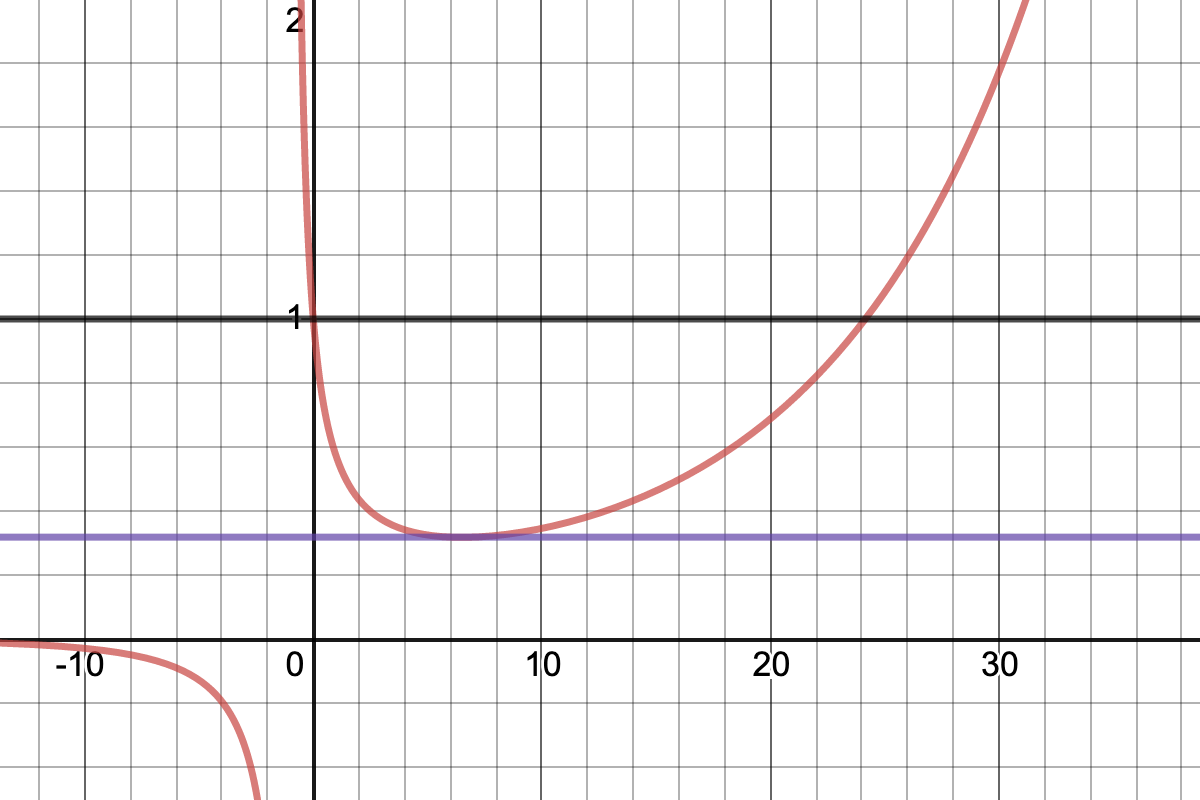
\includegraphics[scale=.2]{graphics/2.5.3.png}}
        \caption{The red line is $y=8^2/(7^2(q+1))$,
        the black line is $y=1$,
        and the purple line is $y=8^2/(7^2(6+1))$
        which is the minimum value Markov's
        inequality gives us for any moment.}
        \label{fig:2.5.3}
    \end{figure}
    \autoref{fig:2.5.3} visualizes the bound
    Markov's Inequality applied to $X^q$ gives.
    The bound gets tighter until $q=6$
    and then looser and becomes vacuous around $q=25$.

    \item
    Define $g(x)$ for $x \in [0,1]$ such that
    $g(x)=0$ if $x<7/8$ and $g(x)=1$ otherwise.
    Then $\E[g(X)] = 0 (7/8) + 1 (1/8) = 1/8$.
    Observe that $g(7/8) = 1$.
    Markov's Inequality gives
    \begin{align}
        \Pr(g(X) \geq g(\frac{7}{8})) =
        \Pr(g(X) \geq 1) \leq E[g(X)] = \frac{1}{8}.
        \nonumber
    \end{align}

\end{enumerate}
